\chapter{微积分}
\centerline{\it “我只能带你到这扇门,你必须自己走进去。”}
\rightline{\it ——墨菲斯,尼布甲尼撒号船长}
\section{总是要从求导开始讲的}
话说在牛顿的时代,大家都喜欢求函数的切线。直觉告诉我们,先画出函数$f(x)$的图像,然后找一个点$(x_0,f(x_0))$,我们可以作一条直线,刚好在这个点上与函数图像相交,而且附近没有第二个交点,如图\ref{fig-tangent}。(注意这个点附近没有第二个交点,别的地方还有交点我们不管)
\begin{figure}[htb]
\centering
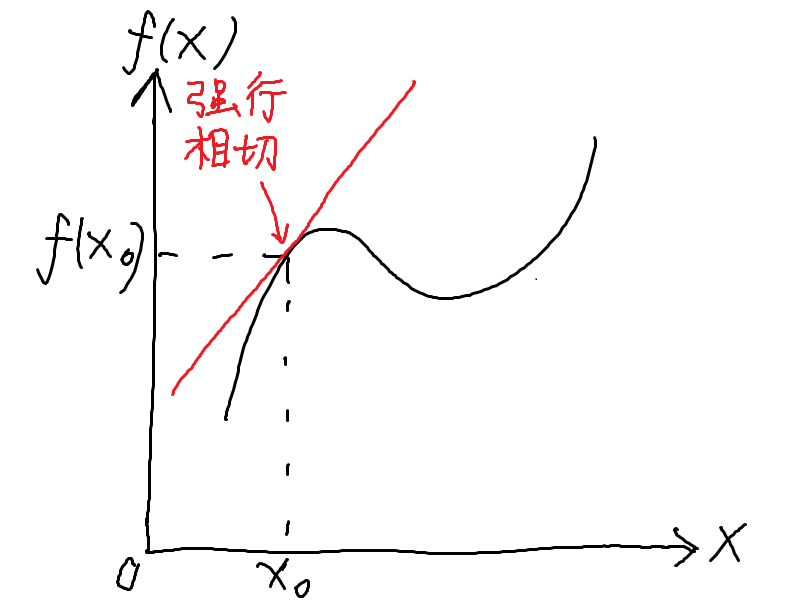
\includegraphics[scale=0.5]{fig/tangent}
\caption{一张灵魂插图}
\label{fig-tangent}
\end{figure}

但是怎么确定这条直线的斜率呢?如果真的只有$x_0$这一个点的话,这条直线是不能确定的,因为两个点才能确定一条直线。但是可以在它旁边再取一个点,然后画一条直线,如图\ref{fig-secant}。
\begin{figure}[htb]
\centering
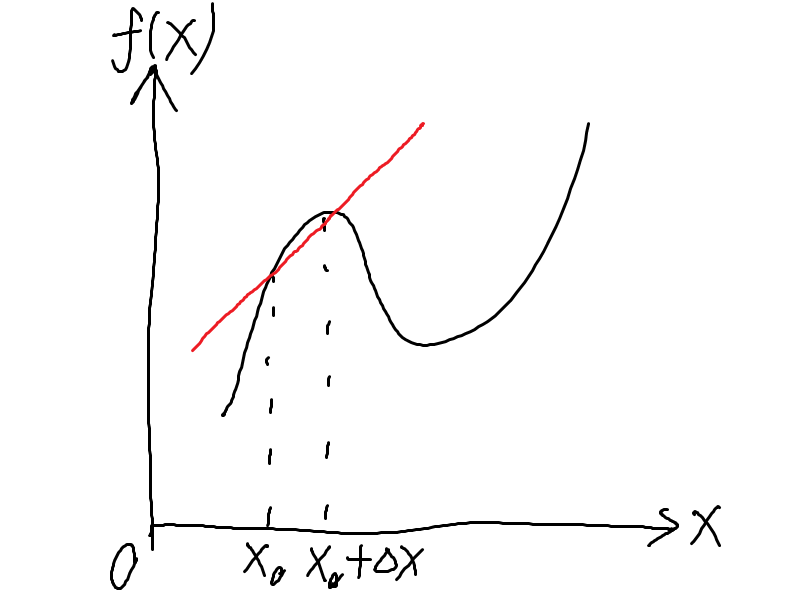
\includegraphics[scale=0.5]{fig/secant}
\caption{每张图下面都有标题是一个好习惯}
\label{fig-secant}
\end{figure}

这条直线的斜率就是$\frac{\Delta f}{\Delta x}=\frac{f(x_0+\Delta x)-f(x_0)}{\Delta x}$。$\Delta x$是一个无穷小的东西,但是它又不是$0$,因为它要出现在分母上。至于无穷小到底是什么意思,有兴趣的同学可以去看高数书上关于极限的内容。

举个栗子:如果$f(x)=x^2$,那么
\begin{align*}
&\mathrel{\phantom{=}}\frac{f(x_0+\Delta x)-f(x_0)}{\Delta x} \\
&=\frac{(x_0+\Delta x)^2-x_0^2}{\Delta x} \\
&=\frac{x_0^2+2 x_0 \Delta x+\Delta x^2-x_0^2}{\Delta x} \\
&=\frac{2 x_0 \Delta x+\Delta x^2}{\Delta x}
\end{align*}

上面这些都是初中就会的东西。然而这时候牛顿干了一件脑洞大开的事情,他说:既然$\Delta x$是一个无穷小的东西,那么$\Delta x^2$肯定比$\Delta x$还小,我们可以不管它。于是上面的式子变成了
\begin{align*}
&\mathrel{\phantom{=}}\frac{2 x_0 \Delta x+\Delta x^2}{\Delta x} \\
&=\frac{2 x_0 \Delta x}{\Delta x} \\
&=2 x_0
\end{align*}

也就是说$\ddx x^2=2 x$。这里$\ddx$表示对$x$求导,然而高中数学课本上把它写成$f'(x)$。

这里有几个名称上的问题需要注意:求导是一个把函数$f(x)$变成另一个函数$f'(x)$的操作,$f(x)$叫作原函数,$f'(x)$叫作导函数,简称导数。$x=x_0$时,$f(x)$的函数值为$f(x_0)$,导数为$f'(x_0)$,也可以写成$\ddx f(x)|_{x=x_0}$,比如$\ddx x^2|_{x=3}=6$。
\section{幂函数的导数}
再试一下$f(x)=x^3$的导数:
\begin{align*}
&\mathrel{\phantom{=}}\frac{(x_0+\Delta x)^3-x_0^3}{\Delta x} \\
&=\frac{x_0^3+3 x_0^2 \Delta x+3 x_0 \Delta x^2+\Delta x^3-x_0^3}{\Delta x} \\
&=\frac{3 x_0^2 \Delta x+3 x_0 \Delta x^2+\Delta x^3}{\Delta x} \\
&=\frac{3 x_0^2 \Delta x}{\Delta x} \\
&=3 x_0^2
\end{align*}

也就是说$\ddx x^3=3 x^2$。

再举一个平凡的例子:如果$f(x)=1$,那么$f(x)$的图像就是一条横线,显然$f'(x)=0$。(平凡的例子有时候很好用)

现在可以猜:对任何正整数$n$,$\ddx x^n=n x^{n-1}$。事实上对任何实数$n$(包括负数、分数甚至无理数),这句话都是对的,前提是$x^n$有定义,当然$-1^{\frac{1}{2}}$之类的东西在实数范围里是没有定义的。目前这句话是猜出来的,稍微严格一些的证明待会再讲。

但是!有一个特殊情况需要注意。$n=0$时,按照上式,$\ddx x^0=0 \cdot x^{-1}=0$。这么说有一定道理,但是严格来说$f'(x)=0$和$f'(x)=0 \cdot x^{-1}$ 的定义域是不一样的。

那么什么东西的导数是$1 \cdot x^{-1}$呢?高中课本告诉我们是$\ln x$,但是这件事情也要待会再讲。

【练习】求证$\ddx x^{-1}=-1 \cdot x^{-2}$,如果能算出来那么之前的东西应该都懂了。
\section{导数与加、减、乘法}
$\ddx(f+g)=\frac{\opd f}{\opd x}+\frac{\opd g}{\opd x}$,这应该很符合直觉。

既然我们知道负数,那么减法就是加法!减法就是加法!!减法就是加法!!!

在上式中令$f=g$,则$\ddx(2f)=\ddx(f+f)=2\frac{\opd f}{\opd x}$。仍然可以猜:$\ddx(c f)=c \frac{\opd f}{\opd x}$,$c$是任何实数。

(再次强调,把正整数改成实数就是为了包含负数、分数和无理数,而$0$经常成为一个特殊情况)(诶我这算是把实数理论讲完了吗)

这两个公式说明,求导这个操作是一个\emph{线性算符}。

(所谓算符就是一种操作,它把一个函数变成另外一个函数,有些地方翻译成算子。线性算符就是满足$L(a f+b g)=a L(f)+b L(g)$的算符,其中$a,b$是实数,$f,g$是函数)

举个栗子,$\ddx(2x^3+3x^2+4x+5)=6x^2+6x+4$,熟练之后这种多项式求导就可以口算了。

两个函数乘起来之后求导就会麻烦一些。可以想象一个长方形,它的一边长是$f(x)$,另一边长是$g(x)$,面积$S(x)=f(x) \cdot g(x)$。现在把两边分别增加$\Delta f$和$\Delta g$,如图\ref{fig-rect}。
\begin{figure}[htb]
\centering
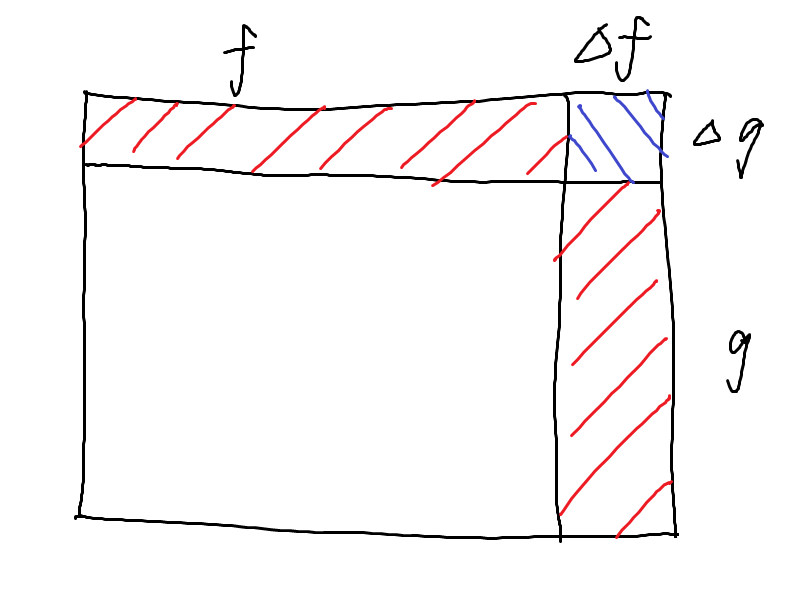
\includegraphics[scale=0.5]{fig/rect}
\caption{长方形的面积改变了多少呢?}
\label{fig-rect}
\end{figure}

$\Delta S=\Delta f \cdot g+f \cdot \Delta g+\Delta f \cdot \Delta g$,然而$\Delta f \cdot \Delta g$比$\Delta f \cdot g$和$f \cdot \Delta g$更小,所以就不管它了。

也就是说,$\ddx(f \cdot g)=\frac{\opd f}{\opd x} \cdot g+f \cdot \frac{\opd g}{\opd x}$。为了\emph{装逼},有些地方把这个公式叫作\emph{莱布尼兹律}。如果$g(x)$是常数$c$,这个公式就是上面乘$c$的公式。

同样我们知道,除法就是乘法!除法就是乘法!!除法就是乘法!!!但是两个函数相除的导数要待会再讲。
\section{$\rme^x$与它的导数;$\rme$到底是什么东西}
有没有一个函数的导数是它自己呢?常函数$f(x)=0$显然是这样的函数。幂函数不是这样的函数,因为求导之后幂指数要$-1$。但是把无穷多个幂函数加起来,就可以构造出这样的函数。

【练习】你可以自己先想一想怎么构造,跟无穷等比数列求和的方法差不多。

比如这个函数:($\exp$是函数的名字,表示exponent,跟$\sin$一样)
\begin{equation*}
\exp x=\sum_{n=0}^{\infty}\frac{x^n}{n!}
\end{equation*}

首先,看到求和号,不要怕,不要怕,不要怕。

这是无穷多个幂函数求和,但是结果并不是无穷大,而是一个有限的数。可以简单判断一下:每一项的分子是$x^n$,分母是$n!$,当$n$很大时,$n! \gg x^n$,每一项都趋于$0$,求和之后确实是一个有限的数。

(“$n$很大”指的是$n \gg x$,大家遇到“很大”“很小”的时候要想清楚谁远大于谁。)

如果把它一项一项写出来就是$1+x+\frac{1}{2}x^2+\frac{1}{6}x^3+\dots$,然后求导,可以发现导数真的跟原函数一样。

但是有一个问题:如果原函数$\times 2$,那么导数也会$\times 2$。如果一个函数满足“导数是它自己”这个要求,那么$\times 2$之后的函数也满足。上面这个$\exp x$的方便之处就在于$\exp 0=1$,所以大家都喜欢用它。可以证明,满足导数是它自己且$f(0)=1$这两个要求的函数有且只有这一个。(这是微分方程的事情,更严格的证明要等到函数空间)

$\exp 1$是一个数学中经常会遇到的数,我们把它叫作$\rme$,这就是高中课本中的$\rme \approx 2.718 \dots$。

有兴趣的同学可以用二项式的一些性质证明$\exp x \cdot \exp y=\exp(x+y)$。以后还可以证明,对任何实数$c$,$(\exp x)^c=\exp(c x)$。这就是指数函数满足的两条性质,所以对任何实数$x$,$\exp x=\rme^x$,它就是大家都知道的以$\rme$为底的指数函数。

有些地方会用另一个极限来定义$\rme$,而这里的定义是从“导数是它自己”这个要求出发的,看起来比较有道理。
\section{多元函数求导;复合函数求导;导数与除法;指数函数的导数}
如果函数$f(x,y)$与自变量$x$和$y$有关(注意现在$x$与$y$无关,或者说我们故意不管$x$与$y$的关系),可以单独对$x$或者$y$求导,只要把其他自变量当作常数就行了。比如$\ddx x^2 y^3=2 x y^3$,而$\ddy x^2 y^3=3 x^2 y^2$。

$\ddx f(x,y)$有时候会写成$\ppx f(x,y)$,来强调这是对多元函数求导。$\partial$称为偏微分算符,其实它和微分算符$\opd$没有什么区别。

($\partial$读作partial,但是很多中国人也会读作偏)

如果对$f(g(x))$这样的复合函数求导,可以把$\frac{\opd f}{\opd x}$拆开来变成$\frac{\opd f}{\opd g} \cdot \frac{\opd g}{\opd x}$。比如:

(诶为什么$f$一会在$\ddx$上面一会在$\ddx$右边呢?这只是书写的习惯问题,意思是一样的)
\begin{align*}
&\mathrel{\phantom{=}}\ddx \ln \frac{1}{x} \\
&=\frac{\opd \ln \frac{1}{x}}{\opd \frac{1}{x}} \cdot \frac{\opd \frac{1}{x}}{\opd x}
\internote{(把$\ln \frac{1}{x}$对“$\frac{1}{x}$”求导,而不是对$x$求导)}
&=\frac{1}{\frac{1}{x}} \cdot -\frac{1}{x^2} \\
&=-\frac{1}{x}
\end{align*}

刚才说过,除法就是乘法。先推导$\ddx \frac{1}{g(x)}=\frac{\opd \frac{1}{g(x)}}{\opd g(x)} \cdot \frac{\opd g(x)}{\opd x}=-\frac{\ddx g(x)}{g^2(x)}$,然后就能得到导数的除法公式$\ddx \frac{f(x)}{g(x)}=\ddx (f(x) \cdot \frac{1}{g(x)})=\frac{\frac{\opd f}{\opd x} \cdot g-f \cdot \frac{\opd g}{\opd x}}{g^2(x)}$。(注意哪个正哪个负!)

按照复合函数求导公式,与$x$相乘的系数在求导的时候可以提到前面,比如$\ddx \rme^{k x}=\frac{\opd \rme^{k x}}{\opd k x} \cdot \frac{\opd k x}{\opd x}=k \rme^{k x}$。

如果是一般的指数函数,$\ddx a^x=\ddx (\rme^{\ln a})^x=\ddx \rme^{\ln a \cdot x}=\ln a \cdot a^x$。
\section{反函数求导;对数函数的导数;填上幂函数的坑}
如果知道$y=f(x)$以及它的导数$\frac{\opd y}{\opd x}=\ddx f(x)$,而$x$可以用反函数$x=g(y)$表示出来,那么$\frac{\opd x}{\opd y}$可以直接用$\frac{1}{\frac{\opd y}{\opd x}}$表示出来。(我不喜欢$f^{-1}(y)$这种写法,会与$f^2(y)$的意思搞混)

比如$y=\exp x$,$x=\ln y$,我们已经知道$\frac{\opd y}{\opd x}=exp x$,那么
\begin{align*}
\frac{\opd x}{\opd y}&=\frac{1}{\frac{\opd y}{\opd x}} \\
&=\frac{1}{\exp x} \\
&=\frac{1}{y}
\end{align*}

也就是说$\ddy \ln y=\frac{1}{y}$。

如果是一般的对数函数,$\ddx \log_a x=\ddx \frac{\ln x}{\ln a}=\frac{1}{\ln a} \cdot \frac{1}{x}=\frac{1}{x \ln a}$。

刚才猜出来,对任何实数$n$,$\ddx x^n=n x^{n-1}$。现在证明:$\ddx x^n=\ddx (\rme^{\ln x})^n=\ddx \rme^{n \ln x}=n \rme^{n \ln x} \cdot \frac{1}{x}=n x^{n-1}$。

\section{三角函数、反三角函数的导数}

首先高中物理课本有这样一句话:$x$(弧度)很小的时候,$\sin x=x$。

(高中里定义三角函数用的是几何方法:如果直角三角形斜边长为$1$,一个角为$x$,那么对边为$\sin x$。和差化积之类的公式也是用几何方法证明的,所以现在看起来不够严谨。刚才用级数定义了指数函数,以后还可以用$\exp \rmi x=\cos x+\rmi \sin x$来定义三角函数。)

我们来看$\sin x$的导数:
\begin{align*}
&\mathrel{\phantom{=}}\sin(x_0+\Delta x)-\sin x_0 \\
&=2 \cos \frac{2x_0+\Delta x}{2} \sin \frac{\Delta x}{2} \\
&=2 \cos \frac{2x_0}{2} \cdot \frac{\Delta x}{2} \\
&=\cos x_0 \cdot \Delta x
\end{align*}

所以$\ddx \sin x=\cos x$。

【练习】证明$\ddx \cos x=-\sin x$,$\ddx \tan x=\frac{1}{\cos^2 x}$(用导数的除法公式)。

三角函数有很方便的性质:$\frac{\mathrm{d^2}}{\opd x^2}\sin x=-\sin x$,$\frac{\mathrm{d^2}}{\opd x^2}\cos x=-\cos x$。($\frac{\mathrm{d^2}}{\opd x^2}$表示对$x$求两次导)

设$y=\sin x$,$x=\arcsin y$,然后来看$\arcsin y$的导数:
\begin{align*}
\frac{\opd x}{\opd y}&=\frac{1}{\frac{\opd y}{\opd x}} \\
&=\frac{1}{\cos x} \\
&=\frac{1}{\sqrt{1-y^2}}
\end{align*}

所以$\ddx \arcsin y=\frac{1}{\sqrt{1-y^2}}$。

【练习】证明$\ddx \arccos x=-\frac{1}{\sqrt{1-x^2}}$,$\ddx \arctan x=\frac{1}{1+x^2}$(需要一些三角变形)。
\section{对方程求导;曲线的切线}
如果把方程的两边对同一个自变量求导,方程仍然成立。

举个栗子:求$x^x$的导数。诶这个东西不是幂函数也不是指数函数,怎么办?可以解方程:
\begin{align*}
y&=x^x
\internote{(既然有指数,可以两边取对数试试看)}
\ln y&=x \ln x \\
\frac{1}{y} \cdot \frac{\opd y}{\opd x}&=\ln x+1
\internote{(注意两边都是对$x$求导,如果左边对$y$求导右边对$x$求导就错了)}
\frac{\opd y}{\opd x}&=y(\ln x+1) \\
&=x^x (\ln x+1)
\end{align*}

这个方法可以求平面内任意曲线(不一定是函数图像)的切线。比如有一个椭圆$\frac{x^2}{a^2}+\frac{y^2}{b^2}=1$,上面有一个点$(x_0,y_0)$,容易算出$y_0=\pm b \cdot \sqrt{1-\frac{x^2}{a^2}}$。可以用黑科技求出过这个点的切线斜率,而不用设直线算$\Delta$之类的:

\begin{align*}
\frac{x^2}{a^2}+\frac{y^2}{b^2}&=1 \\
\frac{2x}{a^2}+\frac{2y}{b^2} \cdot \frac{\opd y}{\opd x}&=0
\internote{(注意$y$与$x$有关,而$a$和$b$是常数)}
\frac{\opd y}{\opd x}&=-\frac{b^2 x}{a^2 y} \\
&=\pm \frac{b x_0}{a \sqrt{a^2-x_0^2}}
\end{align*}

这个斜率前面有$\pm$,因为现在把它表示成$x_0$的函数,而一个$x_0$对应椭圆上的两个点,所以有两条切线,到底是哪一条要看情况判断。
\section{什么样的函数是可以求导的}
到这里为止我们已经可以动手算很多导数了,但是有的函数在某些点根本就不能求导,这种情况在高中是大家都不关心的,但是我们要留个心眼。

常见的人畜无害的函数有幂函数、指数函数、对数函数、三角函数、反三角函数,以及它们经过有限次加、乘、复合构成的函数,它们叫作\emph{初等函数}。初等函数在它们的定义域内都是可以求导的。(无限次复合就会出现奇怪的事情,现在不去管它)

一个函数要求导,首先要求它的图像是连续的,在断掉(比如某些高中数学老师拍脑袋想出来恶心别人的分段函数)的点是不行的,爆掉(趋于$+\infty$或$-\infty$,英文就是blow up)的点也是不行的,如图\ref{fig-bad-deri}。
\begin{figure}[htb]
\centering
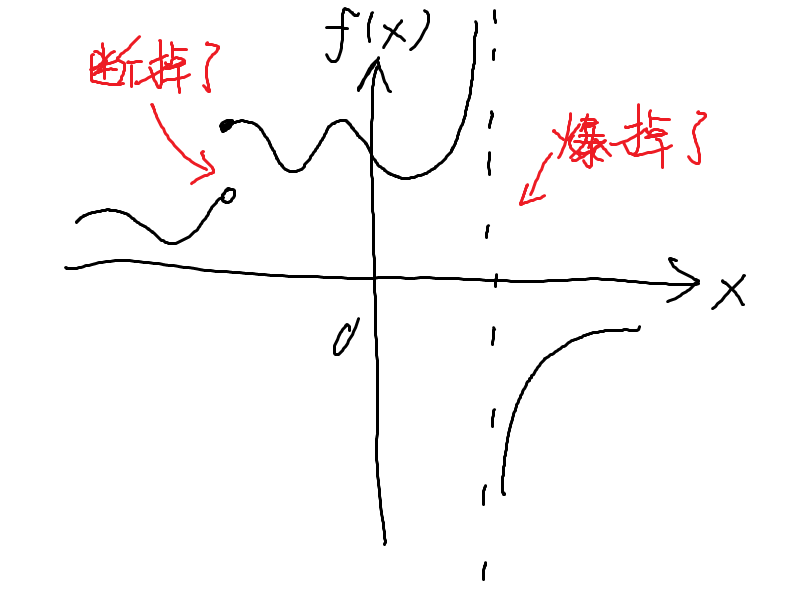
\includegraphics[scale=0.5]{fig/bad-deri}
\caption{画图记得原点和坐标轴的名字}
\label{fig-bad-deri}
\end{figure}

如果分段函数的图像没有断掉,可以算一下两边的导数,如果不同,那么在分割点就不能求导;如果相同,那么分割点的导数就是它了。

比如绝对值函数$f(x)=|x|$,左边的导数是$-1$,右边的导数是$+1$,两边不同,那么$x=0$时就不能求导。而两边导数相同的函数比如(灵魂画师表示懒得画图了,大家自己画吧)
\begin{equation*}
f(x)=
\begin{cases}
2x, &x \le 1 \\
x^2+1, &x>1
\end{cases}
\end{equation*}

那么$\ddx f(x)|_{x=1}=2$。

狄利克雷曾经构造出了处处不连续的函数,而魏尔斯特拉斯构造出了更加丧心病狂的处处连续但不可导的函数。
\section{积分就是导数的逆运算}
把这节的标题读一遍,然后就讲完了。各种奇怪的换元等到要用的时候再讲。如果你对微积分还不熟悉,要注意不定积分和定积分的关系、积分常数,还可以去高数书上看看分部积分法。

悲剧的是,不是所有初等函数的积分都可以算出来(用初等函数表示),比如$\rme^{-x^2}$、$\frac{\sin x}{x}$的积分都是算不出来的。

【练习】自己写一遍幂函数、指数函数、对数函数、三角函数、反三角函数的导数和积分表。
\section{睡前小故事:$\sqrt{-1}$与$\frac{1}{0}$}
在实数范围内,$\sqrt{-1}$是不存在的。然而我们硬要定义$\rmi=\sqrt{-1}$(的一个值),于是就有了复数。那么能不能定义一个$\rmj=\frac{1}{0}$呢?硬要定义的话确实可以,但是这样一来世界上就只剩下一个实数了,我们觉得这样做很不好。

诶这是什么情况?首先来整理一下,实数满足这样几条公理(这里列出的不全,但是够用了):
\begin{enumerate}
\item 存在一种运算叫加法,它把两个实数变成一个实数。(不要小看关于存在性的公理!迟早有一天我们会被存在性坑一发!)
\item $(a+b)+c=a+(b+c)$。(加法结合律)
\item $a+b=b+a$。(加法交换律,以后会发现很多时候结合律比交换律更重要)
\item 存在一个实数叫$0$,使得对任何实数$a$,$a+0=a$。
\item 存在一种运算叫减法,它是加法的逆运算,也就是说对任何实数$a$,$a-a=0$。
\item 存在一种运算叫乘法,它把两个实数变成一个实数。
\item $(a \cdot b) \cdot c=a \cdot (b \cdot c)$。(乘法结合律)
\item $a \cdot b=b \cdot a$。(乘法交换律)
\item 存在一个实数叫$1$,使得对任何实数$a$,$a \cdot 1=a$。
\item 存在一种运算叫除法,它是乘法的逆运算,也就是说对任何不为$0$的实数$a$,$\frac{a}{a}=1$。(“不为$0$”意味着$0$和$1$的地位不一样,加法和乘法的地位也不一样)
\item 乘法分配律。(这是加法和乘法另一个不一样的地方)
\end{enumerate}

而等号满足这样几条公理:
\begin{enumerate}
\item $a=a$。
\item 如果$a=b$,那么$b=a$。
\item 如果$a=b$,$b=c$,那么$a=c$。
\end{enumerate}

诶你怎么还没睡着?所谓公理就是这些看起来像废话的东西,但是所有的证明必须严格按照它们来推导。比如证明任何一个实数乘$0$等于$0$:
\begin{align*}
a \cdot b&=a \cdot b \\
a \cdot (b+0)&=a \cdot b \\
a \cdot b+a \cdot 0&=a \cdot b \\
a \cdot 0&=0
\end{align*}

这件事情符合我们的直觉,而公理也保证了这件事情的严谨性。如果定义一个$\rmi$,这几条公理仍然是满足的,所以大家觉得这件事情很好。

但是!如果定义一个$\rmj$,这几条公理就会出问题,因为它在直接挑战$0$和$1$的地位。

既然定义了$\rmj$,那么除法的定义里的“不为$0$”应该去掉。然后按上面的公理来推导:
\begin{align*}
0 \cdot \rmj&=1 \\
a \cdot (0 \cdot \rmj)&=a \cdot 1 \\
(a \cdot 0) \cdot \rmj&=a \cdot 1 \\
0 \cdot \rmj&=a
\end{align*}

同理可得$0 \cdot \rmj=b$,所以$a=b$。也就是说,世界上只剩下一个实数了。如果硬要让$a \neq b$,那么乘法结合律、乘法分配律或者等号满足的公理就会出问题,那就更不好了。
